\documentclass[final]{fhnwreport}       %[mode] = draft or final
                                        %{class} = fhnwreport, article, 
                                        %          report, book, beamer, standalone
\input{header}			                %loads all packages, definitions and settings											
\title{Fachbericht}  		        %Project Title
\author{Team 1}      				    %Document Type => Technical Report, ...
\date{\today}          				   %Place and Date

\begin{document}

%%---TITLEPAGE---------------------------------------------------------------------------------
\thispagestyle{empty}
%	\ohead{\includegraphics[scale=0.5]{Bilder/Logo_FHNW.jpg}}
	\begin{figure}
		 \vspace*{-\topskip}\vspace*{-\headsep}
		\includegraphics[scale=1]{graphics/fhnw_ht_logo_de.pdf}
	\end{figure}
	\begin{center}
		\vspace*{2cm}
		{\huge{\textbf{digitales Theremin}}}\\
		\vspace*{0.2cm}
		{\huge{\textbf{\thetitle}}}\\
		\vspace*{0.5cm}
		
		{\scshape\Large Projekt 6\\} \Large{\today}
		\vfill
		\begin{normalsize}
			{\begin{tabbing}
					\textbf{Auftraggeber:} \hspace{5cm}\= Prof. Dr. Hanspeter Schmid\\
					
					\\[0.8cm]
					\textbf{Betreuung:} 
					\>Prof. Dr. Hanspeter Schmid\\
					\>Herr Prof. Karl Schenk\\


					\\[0.8cm]
					\textbf{Team:} \>Andreas Frei \\ \>Dennis Aeschbacher \\ 

					\\[0.8cm]
					\textbf{Studiengang:} \>Elektro- und Informationstechnik
					\\[0.8cm]	\textbf{Semester:} \>Frühlingssemester 2020
			\end{tabbing}}
		\end{normalsize}
		\vfill
	\end{center}
\clearpage
			
%%---ABSTRACT----------------------------------------------------------------------------
\selectlanguage{english}				%ngerman or english
\thispagestyle{empty}
\begin{abstract}
% Description aim/objective
\noindent This project was a continuation on the work on a Theremin that mainly operates on digital hardware. Unlike the original device, which solely used analog electronics. The device is supposed to be used in presentations for trade fairs by the Institute for Sensors and Electronics ISE. As such the device should be built in an appealing housing. Moreover the device should have other additional functionality that helps the player to use the instrument more easily.
% Method
The digital hardware was implemented in VHDL on the developer board DE1-SoC from terasIC with a Cyclone V FPGA from Intel. The sole analog component implemented were the oscillators that control the pitch and volume by use of two antennae and the codec, wich converts the audio data for use on a loudspeaker. 
% Results
The pitch and volume of the instrument can be changed by the two antennae like a usual theremin. To adjust settings the theremin has a touchscreen display that is controlled by the Nios system, that was implemented. The theremin has two functionalities, that help the player use the instrument more easily. First the glissando effect, wich corrects the pitch to the closest musical note. Second the pitch display, wich displays the closest musical note the player ist playing at and the deviation that the player is causing.
% Conclusion
In conclusion it can be said, that the theremin is ready for any trade fairs that will come.


\end{abstract}	



%%---TABLE OF CONTENTS-------------------------------------------------------------------
\pagenumbering{Roman}		
\selectlanguage{ngerman}				%ngerman or english
\tableofcontents
\clearpage

%%---TEXT--------------------------------------------------------------------------------
\pagenumbering{arabic}
\clearpage
\section{Einleitung}\label{sec:Einleitung}
Das Theremin kennen heutzutage nur wenige Leute, obwohl es das erste elektronische Instrument war. Es wurde 1920 von dem Russen Lev Sergejewitsch Termen, welcher sich später zu Leon Theremin umbenennen liess, erfunden \cite{Theremin_h}. Personen die regelmässig Filme schauen, haben die Musik welche mit einem Theremin gemacht wird bestimmt schon einmal gehört. Ein Beispiel dafür ist Ghostbusters, wo das Theremin oft im Hintergrund zu hören ist. Zudem ist das Theremin in einigen Science-Fiction-Filmen und Horrorfilmen zu hören \cite{Goast_m}. Das Theremin wird ohne es zu berühren gespielt, indem man mit den Händen die Distanz zu zwei Antennen ändert. Dies führt zu Veränderung der Tonhöhe und Lautstärke.

Im Projekt 5 und 6 soll nun ein solches Instrument entwickelt werden. Mit dem Unterschied, dass das sonst analoge Instrument digital aufgebaut werden soll. Dabei soll es auf einem Field Programmable Gate Array (FPGA) implementiert werden. Später soll das Theremin als Messeobjekt für das Institut für Sensorik und Elektronik ISE verwendet werden. Im Rahmen des Projekt 5 wurde die Tonhöhenantenne des Theremin realisiert. Dazu wurde die Antenne zusammen mit dem Antennenoszillator analog beibehalten. Die restlichen Komponenten wurden in VHDL realisiert. Das Resultat wurde auf dem DE1-SoC Board von terasIC mit einem Cyclone V FPGA von Intel getestet.

Der folgende Fachbericht beginnt mit dem Kapitel \ref{sec:Technische Grundlagen} Technische Grundlagen.In der ersten Hälfte des Kapitel wird erklärt wie ein analoges Theremin funktioniert und welche Komponenten ein Theremin ausmachen. In der zweiten Hälfte werden digitale Lösungsansätze besprochen. Anschliessend wird im Kapitel \ref{sec:Realisierung} Realisierung beschrieben wie die Komponenten realisiert wurden. Im Kapitel \ref{sec:Validierung} Validierung wird als erstes auf die Inbetriebnahme des Antennenoszillators eingegangen. Als nächstes werden die Simulationen des VHDL Codes erläutert. Im letzten Abschnitt wird auf die Inbetriebnahme des VHDL Codes auf dem DE1-SoC Board Bezug genommen.


\todo{Erklärung zu Glissando und Anzeige Spielgenauigkeit}




\pagebreak

	
\clearpage
\section{Technische Grundlagen}\label{sec:Technische Grundlagen}
In diesem Kapitel ist als erstes erklärt wie ein analoges Theremin funktioniert um ein Verständnis für dessen Funktionsweise zu gewinnen. Anschliessend folgt ein kleiner Abschnitt zur Musiktheorie. Zuletzt werden verschiedene Algorithmen erklärt, welche im digitalen Theremin eingesetzt wurden.
	\subsection{Analoges Theremin}\label{subsec:Theremin_analog}
Das klassische Theremin besitzt zwei Antennen. Der Spieler kann über die senkrecht angebrachte Antenne  die  Tonhöhe beeinflussen. Mit der waagrechten Antenne regelt der Spieler die Lautstärke. Eine typische Eigenschaft des Theremins ist, dass der Ton des Theremins in einem weiten Frequenzbereich kontinuierlich veränderbar ist. Das Theremin kann daher alle Frequenzen in einem Bereich spielen, im Gegensatz zu den meisten anderen Instrumenten.

Der Spieler spielt das Theremin durch verstimmen der Oszillatoren über die Antennen.
Die Hand des Spielers verändert über die jeweilige Antenne die Schwingfrequenz des Tonhöhen- und Lautstärkenoszillators. Dabei wird der kapazitive Anteil des LC-Schwingkreises beeinflusst, was eine Änderung der Schwingfrequenz zur Folge hat. 
Die Frequenz dieser Oszillatoren ist jedoch weit über dem hörbaren Bereich (zwischen \SI{100}{kHz} bis \SI{1}{MHz}). Mit Hilfe eines Mischers und einem Referenzoszillator wird die Frequenzdifferenz des Tonhöhenoszillators hörbar gemacht und danach verstärkt\cite{Franzis}. Der Lautstärkepegel ergibt sich durch die Verwendung eines Bandpassfilters und eines nachfolgenden Hüllkurvendetektors. Die Abbildung \ref{img:Blockschaltbild_analog} gibt einen Überblick über die Schaltungskomponenten eines Theremins. Die einzelnen Schaltungsteile sind im folgenden Teil genauer erklärt.

\begin{figure}[h]
	\centering
	\includegraphics[width=0.8\textwidth]{Blockschaltbild_analog.pdf}
	\caption{Blockschaltbild eines analogen Theremins}
	\label{img:Blockschaltbild_analog}
\end{figure}

\paragraph{Tonhöhenoszillator und Tonhöhenantenne}\mbox{}\\

Die Tonhöhenantenne ist ein Metallrohr, welches mit dem Tonhöhenoszillator verbunden ist.
Der Spieler kann über die Distanz seiner Hand zur Antenne die Frequenz des Tonhöhenoszillator verändern. Die über die Antenne zu erreichende Kapazitätsänderung ist sehr gering. Diese liegt im Picofarad Bereich \cite{physik_theremin}. Die Grundfrequenz des Tonhöhenoszillators muss weit über dem hörbaren Bereich liegen, damit eine genügend grosse Frequenzänderung entsteht.

\paragraph{Lautstärkenoszillator und Lautstärkenantenne}\mbox{}\\ 

Die Lautstärkenantenne ist wie die Tonhöhenantenne ein Metallrohr, welches mit dem Lautstärkenoszillator verbunden ist. Die durch den Spieler beeinflusste Frequenzänderung wandelt ein Hüllkurvendetektor in eine Spannung um. Diese Spannung dient dem Verstärker als Steuergrösse, um das Audio Signal zu verstärken. \cite{Franzis}. 

\paragraph{Mischer und Referenzoszillator}\mbox{}\\ 
\\Die erzeugte Frequenz der Tonhöhenantenne liegt weit über dem vom Menschen hörbaren Bereich. Der Mischer multipliziert die Signale des Referenzoszillators und des Tonhöhenoszillators wie in Formel \ref{equ:mischer}. $A_1\sin(\omega_1t)$ entspricht dem Signal des Referenzoszillators und $A_2\sin(\omega_2t)$ dem Signal des Tonhöhenoszillators.

\begin{equation}
V_{out} = A_{1}A_{2} \sin(\omega_{1}t)   \sin(\omega_{2}t) 
\label{equ:mischer}
\end{equation}

$V_{out}$ kann durch Additionstheoreme umgeformt werden. Dabei erhält man folgenden Ausdruck:

\begin{equation}
V_{out} = A/2[\cos((\omega_{1}-\omega_{2})t)  - \cos((\omega_{1}+\omega_{2})t) ]
\label{equ:mischer_trigo}
\end{equation}

Das Ausgangssignal $V_{out}$ hat zwei Frequenzkomponenten. Zum einen die Differenz der beiden Frequenzen, zum anderen die Summe der Frequenzen. Dabei ist bei dem Theremin nur die Differenz der Frequenzen von Interesse \cite{physik_theremin}.

Eine Kalibration des Theremins ist vor jedem Gebrauch nötig. Es könnte beispielsweise sein, dass die Differenz der Frequenz ausserhalb des hörbaren Bereiches liegt. Dazu stellt der Spieler beim klassischen Theremin mit Hilfe eines Trimmkondensators am Referenzoszillator die Differenzfrequenz auf \SI{0}{Hz} ein.

\paragraph{Tiefpassfilter}\mbox{}\\ 
\\Das Tiefpassfilter filtert die hochfrequente Komponente aus Formel \ref{equ:mischer_trigo} weg. Übrig bleibt die Differenz der Oszillatorfrequenzen. Dies ist der interessante Anteil des Mischprozesses, da er im hörbaren Bereich liegt.
\begin{equation}
V_{out} = A/2cos((\omega_{1}-\omega_{2})t) 
\label{equ:mischer_gefilt}
\end{equation}

\paragraph{Verstärker und  Lautsprecher}\mbox{}\\ 
\\Der Verstärker verstärkt das Ausgangssignal des Tiefpassfilters abhängig von der Spannung, welche vom Hüllkurvendetektor stammt.

	\subsection{Musiktheorie}\label{subsec:Musiktheorie}

Um besser an einem Musikinstrument arbeiten zu können, ist es wichtig, ein wenig Musiktheorie zu kennen. Der wichtigste Fakt ist, dass unser Gehör den Schallpegel logarithmisch wahrnimmt. Der Schallpegel wird in Dezibel (dB) angegeben. Auch die Frequenz der Tonhöhe hören wir nicht linear. Ein Ton mit \SI{400}{Hz} nehmen wir nicht als doppelt so hoch wahr, wie ein Ton mit \SI{200}{Hz}. Dies ist sehr schön ersichtlich in Tabelle \ref{tab:Toene_Frequenzen}. Je höher die Töne ansteigen, desto höhere Frequenzunterschiede entstehen zwischen ihnen. Für einfacheres Rechnen dieser Unterschiede ist die Masseinheit Cent gebräuchlich. Dabei ist definiert, dass zwei Töne \SI{100}{Cent} auseinanderliegen und dass zwei Töne mit einer Oktave Unterschied \SI{1200}{Cent} Frequenzunterschied haben. Diese Cent-Werte kann man mithilfe von Formel \ref{equ:Cent} in einen Faktor umrechnen \cite{Cent}.

\begin{equation}
x = \sqrt[\leftroot{-2}\uproot{1}1200]{2}^{n_{cent}}
\label{equ:Cent}
\end{equation} 

Dabei ist \(n_{cent}\) der Unterschied in Cent und \(x\) als Faktor.\\
Wird nun die \glqq akustische\grqq{} Mitte zwischen zwei Tönen gesucht, ist die Berechnung mit Cent nützlich. Diese Mitte liegt nicht linear zwischen den beiden Tönen, sondern \SI{50}{Cent} entfernt von beiden Tönen. Werden diese \SI{50}{Cent} in einen Faktor umgerechnet und mit dem tieferen Ton multipliziert erhält man diese \glqq akustische\grqq{} Mitte.

Um nun zu sagen, wann ein Unterschied in der Frequenz vom Gehör wahrgenommen wird, ist abhängig von dem Gehör der jeweiligen Person. Als Faustformel kann gesagt werden, dass das Gehör zwei aufeinanderfolgende Töne mit etwa \SI{6}{Cent} Unterschied registriert. Jedoch ist es schwierig zu sagen, wann das Gehör einen Ton als \glqq nicht getroffen\grqq{} empfindet \cite{Cent}.

Ein weiteres interessantes Thema ist die Pentatonik. Dabei handelt es sich um ein Tonsystem mit nur 5 Tönen. Ein gutes Beispiel dafür sind die schwarzen Tasten des Klaviers. Benützt der Spieler nur diese Tasten, spielt er in einem pentatonischen Tonsystem. In Abbildung \ref{tab:Toene_Frequenzen} entspricht dies allen Tönen mit einem \# in der Notation. Ein Merkmal der Pentatonik ist, dass es sehr einfach ist eine Melodie zu spielen, die ansprechend klingt, ohne grossen Aufwand \cite{Pentatonik}.



\begin{table}[H]
	\centering
	\caption{Töne aus vier Oktaven und deren Frequenzen \cite{Toene_Frequenzen}}
	\label{tab:Toene_Frequenzen}
	\begin{tabular}{l|l|l|l|l|l}
		\textbf{Ton} & \textbf{Frequenz[Hz]} & \textbf{Ton} & \textbf{Frequenz[Hz]} &\textbf{Ton} & \textbf{Frequenz[Hz]} \\
		\hline\hline
		C3 	& 130.813 	& F4	 & 349.228		& A\#5	 &  932.328	 \\ \hline
		C\#3 & 138.591 	& F\#4	 & 369.994		& B5	 &  987.767	 \\ \hline
		D3 	& 146.832 	& G4	 & 391.995		& C6	 &  1046.5	 \\ \hline
		D\#3 & 155.563 	& G\#4	 & 415.305		& C\#6	 &  1108.73	 \\ \hline
		E3 	& 164.814 	& A4	 & 440		 	& D6	 &  1174.66	 \\ \hline
		F3 	& 174.614 	& A\#4	 & 466.164		& D\#6	 &  1244.51	 \\ \hline
		F\#3 & 184.997 	& B4	 & 493.883		& E6	 &  1318.51	 \\ \hline
		G3 	& 195.998 	& C5	 & 523.251		& F6	 &  1396.91	 \\ \hline
		G\#3 & 207.652 	& C\#5	 & 554.365		& F\#6	 &  1479.98	 \\ \hline
		A3 	& 220 		& D5	 & 587.33		& G6	 &  1567.98	 \\ \hline
		A\#3 & 233.082 	& D\#5	 & 622.254		& G\#6	 &  1661.22	 \\ \hline
		B3 	& 246.942 	& E5	 & 659.255		& A6	 &  1760	 \\ \hline
		C4 	& 261.626 	& F5	 & 698.456		& A\#6	 &  1864.66	 \\ \hline
		C\#4 & 277.183 	& F\#5	 & 739.989		& B6	 &  1975.53	 \\ \hline
		D4 	& 293.665 	& G5	 & 783.991		& C7	 &  2093	 \\ \hline
		D\#4 & 311.127 	& G\#5	 & 830.609		&  		 &  		 \\ \hline
		E4 	& 329.628 	& A5	 & 880		 	&  		 &  		 \\ \hline
	
		
	\end{tabular}
\end{table}
	\subsection{Cordic Algorithmus}\label{subsec:Cordic}

Um in einem FPGA aufwendigere Rechenoperationen wie die Berechnung eines Sinus zu implementieren ist eine zusätzliche Hardware notwendig. Weit verbreitet ist dafür der Cordic Algorithmus. Nebst anderen diversen Rechenoperationen ist der Einsatz als Sinusgenerator möglich, was in späteren Kapiteln genauer besprochen ist. \\
Der Cordic Algorithmus ist ein iterativer Algorithmus, welcher praktisch nur Additionen und Verschiebungen von Bits benötigt. 
Der Algorithmus besitzt zwei Modi. Zum einen der Vektor Modus, in welchem die Berechnung eines Winkels aus einem gegebenen Vektor möglich ist. Zum Anderen der Rotationsmodus, mit welchem die Berechnung der Elemente eines Vektors aus einem gegebenen Winkel möglich ist. Die folgenden Formeln sind für diese Berechnung notwendig \cite{Cordic}:

\begin{equation}
x_{i+1} = x_i - y_id_i2^{-i}
\label{equ:cordic_1}
\end{equation} 
\begin{equation}
y_{i+1} = y_i + x_id_i2^{-i}
\label{equ:cordic_2}
\end{equation} 
\begin{equation}
z_{i+1} = z_i - d_i\arctan{2^{-i}}
\label{equ:cordic_3}
\end{equation} 

\(x_i\) und \(y_i\) sind dabei die Elemente des Vektors und \(z_i\) ist der Winkel des Vektors. \(x_{i+1}\),\(y_{i+1}\) und \(z_{i+1}\) sind die Resultate einer Iteration.
Die Berechnung von \(d_i\) im Rotationsmodus lautet wie folgt: 

\begin{equation}
d_i=
\begin{cases}
-1 &z_i < 0 \\
1 &\text{otherwise}
\end{cases}
\label{equ:cordic_4}
\end{equation} 

Formeln \ref{equ:cordic_1} bis \ref{equ:cordic_3} zeigen schön den iterativen Ablauf des Algorithmus auf. Um nun einen Sinuswert zu berechnen sind folgende Initialwerte notwendig:

\begin{equation}
\begin{aligned}
x_0 = 1 \\
y_0 = 0 \\
z_0 = \varphi
\end{aligned}
\label{equ:cordic_5}
\end{equation} 

\(\varphi\) ist der gegebene Winkel, welcher zwischen \(-\pi/2\) und \(\pi/2\) sein muss, damit der Algorithmus konvergiert.

Daraus ergeben sich nach \(n\) Iterationen der Sinus und Kosinus Wert wie folgt:

\begin{equation}
\begin{aligned}
x_n = \frac{\cos{\varphi}}{A} \\
y_n = \frac{\sin{\varphi}}{A}
\end{aligned}
\label{equ:cordic_6}
\end{equation} 

Schlussendlich ist es notwendig die Resultate um den Faktor \(A = 0.60725294\) zu korrigieren um die richtigen Werte zu erhalten.


	\subsection{CIC Filter}\label{subsec:CIC_Filter}

Ein CIC-Filter oder Cascaded-Integrator-Comb-Filter ist ein digitales Filter, welches nebst der Filterung eines Signals zusätzlich deren Abtastfrequenz verändert. Abbildung \ref{img:CIC_Filter} zeigt ein Dezimations-CIC-Filter. Dieses verkleinert die Abtastfrequenz am Ausgang um den Faktor \(R\). Die zweite Form ist ein Interpolation-CIC-Filter. Dieses vergrössert die Abtastfrequenz um den Faktor \(R\).

In Abbildung \ref{img:CIC_Filter} ist zu sehen, dass das Filter in drei Stufen unterteilt ist. Links ist ein Integrator-Filter zu sehen, welches einen anliegenden Wert mit einem verzögerten Wert aufaddiert oder anders gesagt, das Signal integriert. Anschliessend folgt ein Dezimierer, welcher das Signal um den Faktor R unterabtastet. Zuletzt folgt ein Combfilter. Dieses nimmt den aktuellen Wert und subtrahiert den alten Wert. Ein Interpolation-CIC-Filter erhält man durch tauschen von Integrator-Filtern mit Comb-Filtern und umgekehrt. Weiter ist nun in der Mitte eine Überabtastung nötig.\\
Es ist möglich, mehrere Integrator- und Combfilterpaare zusammen zu schalten, um eine grössere Dämpfung höherer Frequenzen zu bewirken. Das CIC-Filter benötigt jedoch, um zu funktionieren, eine gewisse Anzahl Bits in den Speichern der Verzögerungselemente, welche grösser als die Anzahl Eingangsbits ist. Dieser Effekt nennt sich Bit-Growth und die zusätzliche Anzahl Bits lässt sich wie folgt berechnen \cite{cic_a} \cite{cic_h}.

\begin{equation}
B_+ = \big \lceil Nlog_2RM \big \rceil
\label{equ:cic_bitgrowth}
\end{equation}

Dabei entspricht N der Ordnung des Filters oder wie viele Integrator-Comb-Filterpaare das Filter hat. R ist der zuvor genannte Dezimationsfaktor und M ist die Verzögerung der Speicherelemente.

Das CIC-Filter verstärkt das Eingangssignal zudem um einen Faktor \(G\). Dieser lässt sich wie folgt berechnen:

 \begin{equation}
 G = (R\cdot M)^N
 \label{equ:cic_gain}
 \end{equation}
 
Um nun den Faktor zu berechnen, um welchen man den Ausgang eines CIC-Filter multiplizieren muss, um den Zahlenbereich voll auszunutzen, kann folgende Formel eingesetzt werden:

\begin{equation}
G_+ = G/2^{B_+}
\label{equ:cic_gain+}
\end{equation}

Ein Problem, welches die CIC-Filter mit sich bringen, ist, dass sie in bestimmten Situationen Aliasing erzeugen. Dieses entsteht wenn sich Signalkomponenten zu nahe an den Nullstellen des Filters befinden \cite{CIC_Aliasing}. In Abbildung \ref{img:CIC_Filter_plot} sieht man sehr schön, dass sehr auf die Frequenz des Signals im Vergleich zum verwendeten CIC-Filter geachtet werden muss.


\begin{figure}[h]
	\centering
	\includegraphics[width=\textwidth]{CIC_Filter.pdf}
	\caption{Aufbau eines CIC-Filters N-ter Ordnung}
	\label{img:CIC_Filter}
\end{figure}

\begin{figure}[h]
	\centering
	\includegraphics[width=0.9\textwidth]{CIC_Filter_plot.pdf}
	\caption{Amplitudengang und Phasengang eines CIC-Filters (M = 1, R = 5; N = 2)}
	\label{img:CIC_Filter_plot}
\end{figure}

\clearpage

	
\subsection{Goldschmidt Algorithmus}\label{subsec:Goldschmidt}

Um in FPGAs dividieren zu können, ist es nötig, selber eine solche Operation zu implementieren. Dafür gibt es für verschiedene Anforderungen diverse Algorithmen. Einer davon ist der Goldschmidt Algorithmus. Dieser ermöglicht es iterativ eine Division zweier Zahlen durchzuführen, welche als Resultat auch Nachkommazahlen enthält. Für die Berechnung multipliziert der Algorithmus den Nenner und Zähler wie in Formel \ref{equ:golds_Q} iterativ mit den Faktoren \(F_i\).

\begin{equation}
Q = \frac{Z}{N}\frac{F_1}{F_1}\frac{F_2}{F_2}\frac{F_3}{F_3}\frac{F_{...}}{F_{...}}
\label{equ:golds_Q}
\end{equation}

Offensichtlich verändert dies nicht das Verhältnis des Zählers und Nenners. Für die Berechnung einer Iteration ergeben sich folgende Formeln:

\begin{equation}
F_{i+1} = 2 - N_i
\label{equ:golds_Fi+1}
\end{equation}
\begin{equation}
Z_{i+1} = F_{i+1}\cdot Z_i
\label{equ:golds_Zi+1}
\end{equation}
\begin{equation}
N_{i+1} = N_{i+1}\cdot Z_i
\label{equ:golds_Ni+1}
\end{equation}

\(N_i\) ist der Nenner, \(Z_i\) ist der Zähler und \(F_i\) ist der zuvor erwähnte Faktor der aktuellen Iteration. \(N_{i+1}\),\(Z_{i+1}\) und \(F_{i+1}\) sind die Resultate einer Iteration.

Damit der Algorithmus richtig funktioniert, ist eine Skalierung des Zählers und Nenners notwendig. Dies, da die Werte nur konvergieren, wenn der Nenner zwischen 0 und 1 ist. Will man beispielsweise 2 durch 3 teilen, ist vorgängig eine Skalierung auf 0.5 respektive 0.75 notwendig. Dies ist in der Hardware durch eine einfache Schiebung nach rechts zu bewerkstelligen.


\clearpage
\section{Konzept}\label{sec:Konzept}
Der Aufbau des digitalen Theremins ist sehr ähnlich, wie das des Analogen, jedoch mit einigen Änderungen, um es besser digital aufzubauen. Abbildung \ref{img:Blockschaltbild_digital} zeigt, dass der Lautstärken- und Tonhöhenoszillator nicht mehr einen Sinus sondern ein Rechteck generieren. Wir haben uns deshalb für diese Änderung entschieden, da es so einfacher ist das Signal in das FPGA einzulesen. Dies da kein Analog-Digital-Wandler nötig ist. Weil der Referenzoszillator weiterhin einen Sinus generiert, ergibt die Mischung mit dem Rechteck auch Mischprodukte mit dessen Oberwellen. Da diese aber eine höhere Frequenz haben, ist eine spätere Filterung möglich.\\
Weiter sind die Referenzoszillatoren neu digital. Um nun einen Sinus zu generieren, wählten wir den in Kapitel \ref{subsec:Cordic} behandelten Cordic Algorithmus. Dieser ist besser um verschiedene Frequenzen zu generieren als eine einfache Lookup-Table, und bietet einen grösseren Lerngewinn. Diese Komponente stammt aus dem Projekt 5. \\
Der Mischer multipliziert den Sinus des Referenzoszillators mit dem Rechteck des analogen Oszillators. Auch diese Komponente stammt aus dem Projekt 5.\\
Für das Tiefpassfilter haben wir uns entschlossen, mehrere CIC-Filter und ein FIR-Filter einzusetzen. Das CIC-Filter stammt ebenfalls aus dem Projekt 5. CIC-Filter haben den Vorteil, dass sie ressourcensparender sind als äquivalente FIR-Filter.\\
Wie man sieht, ist die Signalverarbeitung für die Lautstärkenverarbeitung bei diesem Aufbau gleich, wie bei der Tonhöhenverarbeitung. Dafür haben wir uns so entschieden, um dieselben Komponenten nochmals nutzen zu können.\\
Um das Audiosignal zu verstärken, benötigt der Verstärker die Frequenzinformation der Lautstärkenverarbeitung. Diese erhält er vom Block Frequenzmessung. Da die Frequenz des Lautstärkenoszillators bei Veränderung der Distanz zu der Antenne exponentiell ändert, ist keinerlei Umrechnung nötig, um eine exponentielle Lautstärkenänderung zu erzielen.
Anschliessend konvertiert der Digital-Analog-Wandler das verstärkte Audiosignal und gibt es am Lautsprecher aus.\\
Wir entschlossen uns dazu, ein Nios II System einzusetzen, um das Theremin zu bedienen und zu steuern. Dies hauptsächlich, um einen Einblick in den Nios II zu gewinnen und um eine Implementation der Steuerung zu vereinfachen. Für die Interagierung mit dem Theremin wählten wir ein Touch Display. Der Bedienungs und Steuerungs Block (Nios II System) wurde in Abbildung \ref{img:Blockschaltbild_digital} nicht mit anderen Komponenten verbunden, um die Zeichnung übersichtlicher zu gestalten.

Über die Steuerung soll zudem eine automatische Kalibration des Theremins möglich sein. Diese soll die verschiedenen Oszillatoren so aufeinander abstimmen, dass eine Annäherung an die Antennen eine Erhöhung der Tonhöhe und Lautstärke bewirkt.

Es soll zudem möglich sein, den in Kapitel \ref{sec:Einleitung} erwähnten Glissando-Effekt zu aktivieren und auf dem Display die Spielgenauigkeit anzuzeigen. Diese beiden Features werden über den Nios II und das Display gesteuert. Die Übergangszeit des Glissando-Effekts soll zudem einstellbar sein und es soll nebst der normalen Tonleiter auch die pentatonische Tonleiter spielbar sein.

\begin{figure}[h]
	\centering
	\includegraphics[width=\textwidth]{Blockschaltbild_digital.pdf}
	\caption{Blockschaltbild des digitalen Theremins}
	\label{img:Blockschaltbild_digital}
\end{figure}

\clearpage
\section{Realisierung}\label{sec:Realisierung}

Das digitale Theremin ist auf dem Entwicklungsboard DE1-SOC von terasIC aufgebaut. Dieses enthält ein Cyclone V 5CSEMA5 FPGA von Intel. Weiter befindet sich auf dem Board der Audio Codec WM8731 von Wolfson für die Ausgabe an einem Lautsprecher. In Abbildung ... \todo{Referenz auf Blockschaltbild} ist der Aufbau des Digitalen Theremin aufgezeigt inklusive der Peripherie ausserhalb des FPGA.

\todo{Blockschaltbild des gesammten Theremin einfügen}
	\subsection{Tonhöhen- und Lautstärkenoszillator}\label{subsec:Antennenoszilator}
Für die Antennenoszillator Schaltung haben wir uns im Projekt 5 für den Colpitts-Oszillator aus Abbildung \ref{img:colpitts} entschieden. Der Aufbau im Projekt 5 umfasste nur einen Oszillator zur Veränderung der Tonhöhe.

Es handelt sich dabei um einen Colpitts-Oszillator mit einem JFET. Diese Schaltung ist von dem Bauset ''Theremin selber bauen`` von Franzis übernommen. 
Da der im Bauset verwendete JFET nicht mehr bestellbar ist, war ein Wechsel auf den J113 N-Kanal JFET nötig. Die mit LTspice simulierten Werte des J113 glichen stark der original Schaltung, weshalb der Entscheid auf diesen fiel. 
Damit das Sinussignal des Antennenoszillator nicht A/D gewandelt werden muss, haben wir entschieden das Sinussignal in ein Rechtecksignal mit gleicher Frequenz zu wandeln. Dies geschieht mithilfe einer Komparatorschaltung. 
Dieser ist mit \SI{3.3}{V} betrieben da die Logikeingänge des FPGA auf diese Spannung ausgelegt sind. 

Im Projekt 5 wurde als Antenne ein Messing Rohr verwendet. Dieses ist zwischen der Spule L1 und dem Kondensator C5 verbunden. 

Die Ausgangsspannung des Colpitts-Oszillator ist über den Kondensator C11 entkoppelt. Dies entfernt den DC-Anteil. Der Kondensator C11 und die Widerstände R3 und R4 bilden zusammen einen Hochpass. Damit die Oszillator Frequenz von ca \SI{562}{kHz} das Filter passieren kann ist C11 so gewählt das die Grenzfrequenz des Filters bei ca \SI{265}{kHz} liegt. 

Auf dem PCB sind nun im Projekt 6 zwei solche Oszillatoren verbaut: Der Tonhöhenoszillator und der Lautstärkenoszillator. Das PCB ist mit einem \SI{12} {VDC} Schaltnetzteil gespiessen. Der MC7809 Spannungsregler generiert die \SI{9} {VDC} für die Colpitts-Oszillator Schaltungen. Die \SI{3.3} {VDC} für den Komperator erzeugt der LT1117 Spannungsregler. Bei der Wahl der Spannungsregel ist darauf geachtet worden das die erzeugten Spannungen möglichst Störungsfrei und wenig Rippel aufwiesen. Das gesamte Schema der Schaltung ist im Anhang enthalten.

\begin{figure}[h]
	\centering
	\includegraphics[width=\textwidth]{colpitts.pdf}
	\caption{Schema Antennenoszillator. Links Collpitts-Oszillator,rechts Komparatorschaltung}
	\label{img:colpitts}
\end{figure} 

\clearpage



	\subsection{Clock}\label{subsec:Clock}
Die verschiednen Clocks für die Hardwarekomponenten und die CPU werden in zwei PLL Blöcken generiert. Ein Block für die Signalverarbeitung und einer für das Nios System. In Tabelle \ref{tab:clocks} sind alle Frequenzen aufgelistet. \\
Alle Frequenzen welche nicht 50MHz sind ergaben sich daraus, dass die externen Peripherien, welche mit den entsprechenden IP Cores verbunden sind, diese Frequenzen als Vorgabe haben. Weiter benötigen die Komponenten Pitch- und Volume Generation die Frequenz 54Mhz, da deren Frequenz ein vielfaches von 48kHz sein muss.

\begin{table}[H]
	\centering
	\caption{Clockfrequenzen der verschiedenen Komponenten}
	\label{tab:clocks}
	\begin{tabular}{l|l|l}
		\textbf{Komponente} & \textbf{Frequenz} & \textbf{PLL Core} \\
		\hline\hline
		Nios Processor & \SI{50}{MHz} & PLL CPU  \\ \hline
		JTAG Controller & \SI{50}{MHz} & PLL CPU \\ \hline
		Timer & \SI{50}{MHz} & PLL CPU \\ \hline
		SysID & \SI{50}{MHz} & PLL CPU \\ \hline
		DRAM Controller & \SI{50}{MHz} & PLL CPU \\ \hline
		SDRAM & \SI{50}{MHz} & PLL CPU \\ \hline
		LCD Controller & \SI{15}{MHz} & PLL CPU \\ \hline
		LCD Reset & \SI{15}{MHz} & PLL CPU \\ \hline
		Touch Interrupt & \SI{15}{MHz} & PLL CPU \\ \hline
		Touch Busy & \SI{15}{MHz} & PLL CPU \\ \hline
		Touch SPI & \SI{15}{MHz} & PLL CPU \\ \hline
		Audio Config & \SI{12}{MHz} & PLL CPU \\ \hline
		Flash Controller & \SI{25}{MHz} & PLL CPU \\ \hline
		Pitch Generation & \SI{54}{MHz} & PLL Signal-Processing \\ \hline
		Volume Generation & \SI{54}{MHz} & PLL Signal-Processing \\ \hline
		DC-FIFO Input	& \SI{54}{MHz} & PLL Signal-Processing \\ \hline
		DC-FIFO Output	& \SI{24}{MHz} & PLL Signal-Processing \\ \hline
	 	Audio Serializer	& \SI{24}{MHz} & PLL Signal-Processing \\ \hline
	 	Codec	& \SI{12}{MHz} & PLL Signal-Processing \\ \hline
		
	\end{tabular}
\end{table}

	\subsection{CPU}\label{subsec:CPU}
Der eingesetzte Nios Prozessor ist für die Bedienung des Theremin und die Steuerung der Signalverarbeitungshardware zuständig. Die diversen eingesetzten IP Cores sind in den unten stehenden Kapiteln beschrieben.

\paragraph{JTAG, Timer und System ID}\mbox{}\\
Der JTAG IP Core ermöglicht das flüchtige Programmieren des Nios wie auch das Kommunizieren mit selbem für Debugging Zwecke. 
Durch den einsatz des Timer IP Cores erhält der Nios einen Interval Timer um beispielsweise periodisch Interrupts zu generieren. 
In dem System ID IP Core ist die Systemidentifikationsnummer gespeichert. Diese wird benötigt um beim laden der Software sicherzustellen, dass das passende Hardware Image vorhanden ist.
Alle drei Komponenten sind mit Standardeinstellungen in das Nios System eingefügt worden.

\paragraph{Speicher}\mbox{}\\

Der Arbeitsspeicher ist ein externer 64MB SDRAM Chip IS42S16320D von ISSI. Für die Kommunikation mit dem Nios Prozessor ist der SDRAM Controller IP Core zuständig. Für die richtige Funktionsweise müssen der Chip und der Controller mit 
	\subsection{Pitch Generation}\label{subsec:Pitch_Generation}

Die Hauptaufgabe der Komponente Pitch Generation ist es das Audiosignal aus dem Rechtecksignal der Tonhöhenantenne (Pitch Antenna) zu generieren. Pitch Generation nimmt zudem eine Frequenzmessung des Audiosignals vor um diverse Funktionalitäten zu gewährleisten. In Abbildung \ref{img:Blockschaltbild_pitch} ist der Grobe aufbau der Komponente aufgezeigt. Die genaue Erklärung zu den einzelnen Komponenten ist in den folgenden Abschnitten zu finden.


\begin{figure}[h!]
	\centering
	\includegraphics[width=1\textwidth]{Blockschaltbild_pitch.pdf}
	\caption{Blockschaltbild der Custom IP Pitch Generation} 
	\label{img:Blockschaltbild_pitch}
\end{figure}  



\paragraph{Referenzoszillator}

Der Referenzoszillator ist wie in Kapitel ... \todo{Referenz auf Grundlagen digitales Theremin} dafür zuständig ein Sinussignal mit Einer Frequenz ähnlich wie der Antennenoszillator ui generieren. Er generiert diesen wie schon erwähnt mithilfe des Cordic Algorithmus. Er ist aufgeteilt in zwei Komponenten: der Cordic Processor und der Cordic Controller. Wie diese beiden Komponenten miteinander verbunden sind ist in Abbildung \ref{img:Referenceoscillator} ersichtlich. \\

Der Cordic Processor berechnet einen Sinuswert aus ...

Der Cordic Controller berechnet den Winkelwert phi in der Form von Abbildung ... \todo{referenz Bild phi einfügen}. 

\begin{figure}[h!]
	\centering
	\includegraphics[width=0.53\textwidth]{Referenceoscillator.pdf}
	\caption{Aufbau des Referenzoszillators} 
	\label{img:Referenceoscillator}
\end{figure}  

\todo{Bild phi einfügen}

\paragraph{Filter}

\begin{figure}[h!]
	\centering
	\includegraphics[width=1\textwidth]{Filter_pitch.pdf}
	\caption{Aufbau des Filters in der Komponente Pitch Generation} 
	\label{img:Filter_Pitch}
\end{figure}  

\paragraph{Frequenzmessung, Kalibration \& Glissandoeffekt}

Die Komponente Frequency Measurement hat mehrere Aufgaben und ist diejenige Komponente mit welcher über den Nios Prozessor die gesammte Pitch Generation gesteuert werden kann. Der Aufbau dieser Komponente ist in Abbildung \ref{freq_meas_pitch} aufgezeigt.\\
Zum einen wird hier die Frequenzmessung durchgeführt. Dies geschieht über die drei Komponenten FIR, Period Counter und Goldschmidt divider. FIR ist wie der Name sagt ein FIR Filter. Dieses ist nötig um das Signal aus dem Filter, welches noch Hochfrequente Signale enthält zu Filtern. Das Filter hat eine Grenzfrequenz von ... \todo{Grenzfrequenz und Dämpfung einfügen}. Das Filter wurde mit dem Tool filterDesigner in Matlab berechnet. Wir haben entschieden die Filterkoeffizienten als fixed-point signed Zahlen in einem Array mit \SI{18}{bit} länge abzuspeichern. Auf dieser Koeffizientenlänge kann Quartus die DSP-Blöcke so nutzen, dass nach der Multiplikation des Signals mit den Koeffizienten die Resultate gleich in den Blöcken addiert wird. Dies ermöglicht längereMultiplikationsketten. \todo{Nochmal über DSP blöcke nachlesen und referenzieren} \\
Anschliessend wird das Signal \textit{fir_out} im \textit{Period Counter ausgemessen}. Diese zählt von Nulldurchgang zu Nulldurchgang einen Zähler hoch. Bei einem Nulldurchgang wird der Wert dieses Zählers am Signal \textit{per_cnt} ausgegeben. Der Zählerwert entspricht der Anzahl Abtastwerte des Signals in einer Signalperiode. \\
Das Signal hat eine Abtastfrequenz von \SI{1.2}{MHz}. Dividiert man diese Abtastfrequenz durch die zuvor gezählte Anzahl Abtastperioden erhält man die Frequenz des Signals.

\begin{figure}[h!]
	\centering
	\includegraphics[width=1\textwidth]{freq_meas_pitch.pdf}
	\caption{Aufbau der Frequenzmessung, Kalibration und Glissandoeffekt in der Komponente Pitch Generation} 
	\label{img:freq_meas_pitch}
\end{figure}  
\todo{Bild überarbeiten und namen an Signalen anbringen wie in Text}
	\subsection{Lautstärkeverarbeitung}\label{subsec:Volume_Generation}
Die Aufgabe der \textit{Lautstärkenverarbeitung} ist es aus dem Signal des Lautstärkenoszillators einen Dämpfungsfaktor zu berechnen, mit welchem das Signal der Tonhöhenverarbeitung multipliziert wird. So kann der Spieler die Lautstärke während dem Spielen wie die Tonhöhe über eine Antenne einstellen. Wie Abbildung \ref{img:Blockschaltbild_volume} zeigt sind die beiden Verarbeitungskomponenten auch sehr ähnlich. Der Referenzoszillator und der Mischer sind gleich wie in der Tonverarbeitung. In den nächsten Abschnitten sind die Unterschiede zu den Komponenten der Tonverarbeitung aufgezeigt.



\begin{figure}[h!]
	\centering
	\includegraphics[width=1\textwidth]{Blockschaltbild_Volume.pdf}
	\caption{Blockschaltbild der Custom IP Volume Generation} 
	\label{img:Blockschaltbild_volume}
\end{figure}  

\paragraph{Filter}\mbox{}\\
Beim \textit{Filter} der Laustsärkeverarbeitung wurde die Frequenzmessung erst nach dem dritten CIC Filter angeschlossen. Wir haben dies so gemacht, um beim FIR-Filter der Frequenzmessungskomponente weniger Koeffizienten und somit weniger Ressourcen zu benötigen. Das FIR-Filter benötigt deshalb weniger Koeffizienten, da nach CIC 3 die Abtastfrequenz des Signals um den Faktor 45 kleiner ist. Zudem ist das FIR-Filter in dieser Komponente deshalb nicht mehr nötig.

\begin{figure}[h!]
	\centering
	\includegraphics[width=0.8\textwidth]{Filter_volume.pdf}
	\caption{Aufbau des Filters in der Komponente Volume Generation} 
	\label{img:Filter_Volume}
\end{figure}  

\paragraph{Frequenzmessung \& Kalibration}\mbox{}\\
Auch bei der Komponente \textit{Frequenzmessung} waren Anpassungen nötig.

\begin{figure}[h!]
	\centering
	\includegraphics[width=1\textwidth]{freq_meas_volume.pdf}
	\caption{Aufbau der Frequenzmessung und Kalibration in der Komponente Volume Generation} 
	\label{img:freq_meas_volume}
\end{figure}  
	\subsection{Audioserialisierer}\label{subsec:Audio_Serializer}

Für die Übertragung der Audiodaten zum Codec ist der \textit{Audioserialisierer} zuständig. Obwohl es von Intel bereits eine IP gäbe, um diese Übertragung zu übernehmen, mussten wir diese Komponente nochmals selber schreiben. Dies, da wir sicherstellen mussten, dass die Clocks dieser Komponente und der Tonhöhenverarbeitung vom selben PLL generiert werden, da ansonsten Werte übersprungen oder verloren gehen. Leider kann die IP von Intel nur mit \SI{12.288}{MHz} betrieben werden. Der IP Core kann jedoch nicht eine solche Frequenz und die gewünschten \SI{54}{MHz} für die Tonhöhenverarbeitung in einem PLL generieren.\\
Wie der Name der Komponente schon sagt serialisiert sie die Parallelen Daten für die Übertragung. Dabei sieht der geforderte Signalverlauf des Codec wie in Abbildung \ref{img:Codec_Signals} dargestellt aus. Der Audioserialisierer gibt jeweils für den linken und rechten Kanal dieselben Daten aus. Die Signale DACLRC und BCLK werden vom Codec nach der Konfiguration beschrieben in Kapitel \ref{subsec:audio} vom Codec generiert und sind Eingänge des Audioserialisierers. Bei jeder positiven Flanke lädt der Serialisierer einen neuen Audiosignalwert ins Schieberegister und schiebt bei jeder negativen Flanke des BCLK ein neues Bit ins Signal DACDAT.

\begin{figure}[h!]
	\centering
	\includegraphics[width=\textwidth]{Codec_Signals_Serializer.pdf}
	\caption{Signalverlauf des Codec Interface} 
	\label{img:Codec_Signals}
\end{figure}  


\pagebreak

\clearpage
\section{Realisierung Software}\label{sec:Realisierung_Software}
Im folgenden Teil des Fachberichtes ist der Aufbau der Software beschrieben. Es folgt zu Beginn eine Gesamtübersicht.

Die Software ermöglicht die Bedienung des Theremin. Zur Steuerung des Theremin ist auf dem NIOS II eine in C programmierten Statemachine realisiert. Die Bedienung geschieht über das LT24 LCD touch module von Terasic. Die von Terasic zur Verfügung gestellten C Dateien zur Ansteuerung des LCD und des Touch, sowie die Dateien zur Darstellung des GUI, stellten sich als wenig brauchbar heraus. Die darin enthaltenen Funktionen sind oft zu ineffizient. Daher entschieden wir uns diese Funktionen selber zu schreiben.
	\subsection{Hauptprogramm State Machine}\label{subsec:State_Machine}
Abbildung bla zeigt die Initialisierung und den Hauptprogrammfluss der Software.
\begin{figure}[h]
	\centering
	\includegraphics[width=\textwidth]{state_machine.pdf}
	\caption{State Machine und Initailisierung.}
	\label{img:Blockschaltbild_digital}
\end{figure}

In der Initialisierung werden als erstes alle Treiber, der Touch, das LCD, und der Codec, und  konfiguriert. Anschlissend wird in einer Endlosschlaufe die state machine aufgerufen.

\textbf{Main}:
Dies ist der erste State nach dem Initialisierungsvorgang. In diesem State wird gewartet bis der Benutzer einer der drei in Abbildung bla gezeigten Tasten drückt. Danach wird je nachdem welcher Taster betätigt wurde in den entsprechende State gewechselt. 
 
\textbf{Calibration}:
Im Calibration State wird der Benutzer gebeten seine Hände in die Nähe der Antenne zu halten.
Nach zwei Sekunden wird die Kalibrierung gestartet. Sobald die Kalibrierung abgeschlossen ist kann der Benutzer über den \textbf{\textit{back}} Taste zurück in den Main State gelangen.  

\textbf{Volume}:
In diesem State kann der Benutzer die Lautstärke ändern und die Volume Antenne aktivieren und deaktivieren. Die Lautstärke kann in 10 verschiedene Pegel eingestellt werden. Dies geschieht mithilfe der in Abbildung bla gezeigten \textbf{\textit{+}} und \textbf{\textit{-}} Tasten. Beim betätigen der \textbf{\textit{vol antenna}} taste wird die Volume Antenne je nach aktuellem Zustand deaktiviert oder aktiviert. Mit dem betätigen der \textbf{\textit{back}} Taste gelangt der Benutzer in den Main State.
 
\textbf{Play Help}:
Im State Play Help kann mit der\textbf{\textit{Glissando on}} Taste der Glissando Effekt akieviert und deaktiviert werden. Über die \textbf{\textit{Set}} Taste gelangt man in den State Settings. Durch betätigen des \textbf{\textit{display pitch}} Taste wird in den State Pitch Display gewechselt.  Mit dem betätigen der \textbf{\textit{back}} Taste gelangt der Benutzer in den Main State.

\textbf{Settings}:
Im Settings State können Einstellungen zum Glissando Effekt gemacht werden. Das Delay des Glissando Effekts kann in 10 Stufen eingestellt werden. Zudem kann mit dem Taster \textbf{\textit{penta}} zwischen der Pentatonischer und der normalen Tonleiter gewechselt werden. Mit dem betätigen der \textbf{\textit{back}} Taste gelangt der Benutzer in den Main State.

\textbf{Pitch Display}:
Im Pitch Display State kann der Benutzer sehen welcher Ton gespielt wird. Ist die Pentatonische Tonleiter aktiv wird angezeigt wie weit man von einem Ton entfernt ist. Falls die normale Tonleiter aktiv ist wird der Ton angezeigt bei welchem man sich am nächsten befindet.


	\subsection{Treiber}\label{subsec:drivers}
In diesem Unterkapitel sind die verschiedenen Funktionen der selbst geschriebenen Treiber für die Custom IP componenten Pitch generation und Volume generation beschrieben. Zusätzlich war die Erstellung  eines Treiber für den LT24 Controller nötig, da Terasic den zur Verfügung gestellte Treiber nicht nach dem Konventionen von Intel erstellt hat.

Um ein selbst erstellten Treiber dem Board Support Package (BSP) hinzuzufügen, müssen  die Benennungen und Ablage Orte der Files einige Bedingungen einhalten.  
 Die Treiber Dateien müssen in einem Ordner IP abgelegt sein, welcher sich im quartus Ordner befinden muss. Darin muss ein Skript mit der Endung sw.tcl abgelegt sein. In diesem Skript muss ein eindeutiger Name für den Treiber angegeben sein. Zudem muss der Pfad zu den Treiber Daten angegeben sein. Intel empfiehlt drei Treiber Daten zu erstellen:
  \renewcommand{\labelitemi}{$\blacksquare$}
 \renewcommand\labelitemii{$\square$}
 \begin{itemize}
 	\item  inc
 	\begin{itemize}
 		\item  custom\_ip\_regs.h
 	\end{itemize}
 \end{itemize}
 \begin{itemize}
	\item  HAL
	\begin{itemize}
		\item  custom\_ip\_.h
		\item  custom\_ip\_.c
	\end{itemize}
\end{itemize}

  Das file mit der Endung regs.h definiert hardware interface spezifische Abläufe. Dieses wird im Ordner inc abgelegt. Im HAL Ordner sind ein c und ein h file erstellt, welche die Integration mit dem hardware abstracten layer(HAL) ermöglichen \cite{NIOS_II_soft}.
 Die folgenden Paragraphe zeigen die in den c Dateien realisierten Funktionen für die drei Treiber.
\paragraph{LT24 Controller}

Wie in der Einleitung dieses Unterkapitels erwähnt erfüllt der von Terasic mitgelieferte Treiber nicht die Konventionen welche Intel verlangt. Zudem sind die meisten Funktionen des Treibers sehr ineffizient gestaltet. Darum haben wir uns entschieden den Treiber für den LT24 Controller selbst zu schreiben. Im folgenden Teil ist beschrieben welche Funktionen wir für die Steuerung des LCD erstellt haben.

Das Mudul \textbf{LT24\_Controller.c} ermöglicht es auf dem LCD einzelne Pixel und Rechteckflächen zu zeichnen und zu löschen. Die Funktion \textit{LCD\_DrawPoint(x,y,color)} setzt ein Cursor an die gewünschte Stelle auf dem LCD und zeichnet ein Pixel in der entsprechenden Farbe. Auf diese Art ein Rechteck zu zeichnen ist sehr ineffizient. Da der Treiber von Terasic Rechtecke auf diese Art zeichnet, haben wir entschieden eine bessere Lösung zu finden. Mit der Funktion \textit{LCD\_DrawRect(xs,ys,xe,ye,color)}  werden Rechtecke effizienter gezeichnet. Es wird dabei nur einmal für das ganze Rechteck ein Cursor Feld gesetzt und danach alle Pixel eingefärbt. Da durch das setzen des Cursor Feld nicht für jeden einzelnen Pixel ein Cursor gesetzt werden muss, wird  Zeit eingespart. Dadurch ist es für das Menschliche Auge nicht mehr ersichtlich wie einzelne Pixel gezeichnet werden, wie dies bei der Funktion von Terasic der Fall ist. 

\paragraph{Pitch generation}
Das Modul \textbf{Pitch\_generation.c} ermöglicht auf das Kontroll und das Glissando Delay Register zu schreiben und diese zu lesen. Das Register freq data ist nur lesbar. Dieses liefert die aktuelle Frequenz der Pitch Antenne und der Index des Tones bei dem die Frequenz am nächsten liegt. 
Die Funktion \textit{get\_pixel\_pitch\_accuracy(penta\_on\_off,pitch\_freq)} liesst das freq data Register aus. Für den Modus Pitch Display, zu sehen in Abbildung \ref{img:play_help_screen}, ist es nötig anzuzeigen auf welcher Seite sich der Benutzer von einem Ton befindet. Daher wird in dieser Funktion das Verhältnis der aktuellen Pitch Antenna Frequenz mit dem Abstand zum nächsten Ton gebildet. Mit diesem Verhältnis wird ein Pixel Wert berechnet. Dieser wird gebraucht um denn vertikalen Strich auf dem LCD zu zeichnen.


\paragraph{Volume generation}
Die einzige Kominikation welche die Volume generation Komponente mit dem NIOS II hat, ist das schreiben und lesen des Kontroll Registers um die Kalibrierung zu starten. Das Module  \textit{Volume\_generation.c} ermöglicht dies. 
	\subsection{Audio}\label{subsec:audio}

Die Kommunikation mit WM8731 Codec geschieht über die IP Componente Audi\_Video Configuration von Intel. Diese besitzt die Funktion 
\textit{alt\_up\_av\_config\_write\_audio\_cfg\_register} um die Kontrollregister des Codec über den Hardware Abstraction Layer (HAL) anzusprechen. \todo{Quelle Intel hinzufügen}.
Das Module \textbf{audio.c} beinhaltet die beiden Funktionen, \textit{codec\_wm8731\_init()} und \textit{set\_vol(vol\_gain)}. 

In der Initialisierung wird der Codec als Master konfiguriert \todo{Verweiss auf Dennis}. Der Clock des Codec wird auf \SI{12}{MHz} gesetzt und die Sampling Rate auf \SI{48}{kHz}. Die Input Audio Data Bit Länge wird auf 24 Bit gesetzt und der Übertragungsmodus der Daten auf left justified gesetzt. Mit diesen Einstellungen ist eine Kominikation mit der audio serializer Komponente möglich \todo{Verweiss auf Dennis}.
Um Störungen zu vermeiden sind die Line In Eingänge des Codec gemutet, da wir nur den Line Out brauchen. Der Linke und Rechte Kanal sind so eingestellt das beide Kanäle die selben Lautstärken haben\cite{codec}. 

Die Gesamtlautstärke des Theremin ist auf 10 unterschiedliche Pegel einbestellbar, dies geschieht mit dem Aufruf der Funktion \textit{set\_vol(vol\_gain)}. Die leiseste Stufe dämpft den Audio Signal Pegel um \SI{-76}{db}. Jeweils eine Stufe grösser reduziert die Dämpfung um \SI{7}{db}. Die höchste Stufe dämpft den Audio Signal Pegel um \SI{-7}{db}. Der Codec könnte gemäss Datenblatt das Signal bis +6dB verstärken. Nach Labor Tests haben wir uns entschieden das Audio Signal nur zu dämpfen, da eine Verstärkung zu laut ist.


Ursprünglich war geplant die Lautstärke Einstellung der Volume Antenne über den Codec zu steuern. Nicht wie in Kapitel \todo{Dennis} beschrieben über die VHDL Komponente. Diese Methode konnte jedoch nicht realisier werden, da die Zero Cross detection des Codec nicht funktionierte. Mit der Zero Cross Dedection sollte der Codec erst bei einem Nulldurchgang die Lautstärke vermindern oder erhöhen. In unseren Versuchen hat sich die Lautstärke jedoch nie geändert, obwohl ein Sinus Audio Signal angelegt wurde. Wir mussten feststellen das diese Methode für den DAC nicht funktioniert. Mit dieser Methode hätte die Lautstärke, verglichen zur realisierten Methode, eine bessere Dynamik gehabt. 
	\subsection{Touch}\label{subsec:touch}
 Die von Terasic zur Verfügung gestellte Datei zum Auslesen des Touch ist leider sehr unübersichtlich aufgebaut. Es ist sehr schwierig, die darin enthaltenen Funktionen auf das Projekt anzuwenden. Daher erstellten wir selbst eine Touch Interrupt Routine. 
 
 Der resistive Touch Display des LT24 LCD Touch Modul ist mit dem AD783 Analoge Devices Chip verbunden. Abbildung \ref{img:AD783_Signalverlauf} zeigt den Signalverlauf des AD783.  Sobald der Touch Display berührt wird, löst der Chip am Pen Interrupt Pin ein Interrupt aus, welches vom Nios II detektiert wird. Darauf schreibt der Nios II über die DIN Leitung ins Kontrollregister um eine Messung der X und Y Koordinaten anzufordern. Während des Acquistation Mode werden die X und Y Koordinaten gespeichert und nach der fallenden Flanke des BUSY Signals über die DOUT Leitung dem Nios II übertragen \cite{AD7843}. 
 
 Für unser Projekt ist es wichtig den Pen Interrupt zu detektieren und die X und Y Koordinaten auszulesen. Auf diese Weise können wir sagen, welche Taste gedrückt worden ist.
 
Das Ganze ist im Modul \textit{touch\_isr.c} realisiert. Darin befindet sich eine Funktion \\ \textit{touch\_init(void*context)}. Diese aktiviert das Touch Pen Interrupt  und registriert die Funktion, welche durch das Interrupt aufgerufen wird. 
In der Interrupt Service Routine\\ \textit{touch\_isr(void*context)} wird zuerst das Touch Pen Interrupt  deaktiviert. So dass in dieser Zeit kein weiteres Interrupt auftreten kann. Nach dem Deaktivieren des Interrupts liesst der \textit{alt\_avalon\_spi\_command} die X und Y Koordinaten aus.

\begin{figure}[h!]
	\centering
	\includegraphics[width=\textwidth]{touch_signal.pdf}
	\caption{Signalverlauf des AD783} 
	\label{img:AD783_Signalverlauf}
\end{figure}  
	\subsection{GUI}\label{subsec:gui}
Die Funktionen, welche von Terasic für die Gestaltung des GUI zur Verfügung gestellt werden, sind für unser Projekt zu ineffizient. Um einen Text anzuzeigen, verwendet Terasic eine Funktion, die ein Alpha Blending an den Rändern der Buchstaben durchführt. Dabei wird die Schriftfarbe mit der Hintergrundfarbe gemischt. Dieser Prozess nimmt viel Zeit in Anspruch und hat wenig Nutzen. Wodurch bei jedem neuen Zeichnen eines Texts zugeschaut werden konnte, wie die Pixel gezeichnet wurden. Dies ist für unser Projekt unbrauchbar. Zudem war eine ansprechendere Schriftart nötig. Daher realisierten wir eine eigene Funktion, welche Texte zeichnet. Diese ist im Modul \textbf{simple\_text.c} umgesetzt.

\paragraph{simple\_text.c}\mbox{}\\

Mit dem Open Source Tool \textit{The Dot Factory} liess sich eine Bitmap für die Schrifftart Arial generieren, welche 22 Punkte gross gewählt ist. Das Tool generiert zwei Arrays. Im Bitmap Array sind die Buchstaben in einer Bitmap gespeichert. Das Descriptor Array enthält Informationen über die Breite jedes Characters und den Offset in der Character Bitmap. Um den Offset eines Buchstabens zu bestimmen, wird der Character minus des ersten Characters in der Bitmap gerechnet. Dies ergibt den Index für das Descriptor Array, in welchem der Offset für die Bitmap gespeichert ist. In Abbildung \ref{img:bitmap} ist dieser Prozess veranschaulicht. In diesem Beispiel besteht die Bitmap aus den Buchstaben a, b und c. Für den Buchstaben b wird der Offset 1 ausgerechnet. Im Descriptor Arrey ist auf Position 1 die Breite 5 gespeichert und der Offset 10 für die Bitmap. Mit diesen Informationen kann die Funktion \textit{print\_string(x,y,color,font,font\_descriptor,string)} einen Text String zeichnen. Dabei werden nur die Pixel gezeichnet, welche in der Bitmap auf 1 gesetzt sind.

\begin{figure}[h]
	\centering
	\includegraphics[width=0.8\textwidth]{the_dot_factory.pdf}
	\caption{Bitmap und Discriptor Array.}
	\label{img:bitmap}
\end{figure}

\paragraph{gui.c} \mbox{}\\

In diesem Modul sind mit der Funktion \textit{print\_string(x,y,color,font,font\_descriptor,string)} aus dem Modul  \textit{simple\_text.c} und der Funktion \textit{LCD\_DrawRect(xs,ys,xe,ye,color)} aus dem Modul \textit{LT24\_controller.c} die einzelnen Menüs dargestellt. 
\pagebreak

\clearpage
\section{Realisierung Gehäuse}\label{sec:Realisierung Gehäuse}
Im folgenden Teil des Fachberichtes ist die Realisierung des Gehäuse beschrieben. 

Die Anforderungen an das Gehäuse des digitalen Theremin sind:
\begin{itemize}
	\item Die Lautstärke- und die Tonhöhenantenne müssen genügend Abstand zueinander haben, damit der Spieler das Theremin richtig spielen kann.
	\item Das Antennenoszillator PCB und das DE1-SoC Board müssen für den Spieler ersichtlich sein.
	\item Für die Bedienung muss das LT24 Touch Modul für den Benutzer gut sichtbar platziert sein.
	\item Um den Preis des Gehäuses tief zu halten und für die Gestaltung des Gehäuses möglichst viel Freiheit zu haben, soll das Gehäuse 3D-gedruckt sein.  
\end{itemize}

Um diese Anforderungen zu erfüllen entschiedenen wir uns das Gehäuse mit dem 3D-CAD-System Inventor zu konstruieren. Inventor ist eine sehr umfangreiche Konstruktion Software mit dem die ausgefallene Form des Gehäuses leicht zu realisieren war.
Um das Gehäuse zu drucken hatten wir uns entschieden den S5 Ultimaker 3D Drucker zu verwenden, da dieser sehr benutzerfreundlich ist und ein grosses Druckvolumen hat. 
Der S5 Drucker hat eine Druckvolumen von \SI{330x240x300}{mm}. 
Das Gehäuse musste jedoch in vier Teile unterteilt werden, damit es im Drucker platz hatte. 

Wir entschieden uns die Form des Theremin oval zu gestalten, da andere kommerziell erhältliche Theremin eine solche Form haben. Die vier Einzelteile des Gehäuses sind alle gleich aufgebaut. Abbildung \ref{img:grundteil} zeigt die Grundstruktur eines Einzelteil. Die Funktion Wandung von Inventor ermöglichte es die Grundstruktur oval auszuhöhlen. Jeweils zwei Einzelteile bilden zusammen den Deckel und den Boden. Daraus resultierte das in Abbildung \ref{img:Theremin_case} gezeigte Gehäuse. 

Die vier Einzelteile sind aus schwarzem Polylactide (PLA)  gedruckt. Da das Gehäuse eine ovale Geometrie hat, braucht es Stützstrukturen für den Herstellungsprozess. Das eingesetzte Polyvinylalkohol (PVAL) hat die nützliche Eigenschaft das es wasserlösslich ist.
\begin{figure}[h]
	\centering
	\includegraphics[width=\textwidth]{grundteil.pdf}
	\caption{Grundstruktur eines Einzelteils.}
	\label{img:grundteil}
\end{figure}
\begin{figure}[h]
	\centering
	\includegraphics[width=\textwidth]{Theremin_case.pdf}
	\caption{Theremin Gehäuse.}
	\label{img:Theremin_case}
\end{figure}





\pagebreak

\clearpage
\section{Validierung}\label{sec:Validierung}
In diesem Kapitel sind die Resultate der Messungen des PCB, der Frequenzmessung, des Glissando-Effekts und des Ton- Display aufgeführt. Dabei werden jeweils der Messaufbau beschrieben und die Resultate dargestellt und kommentiert. 
	\subsection{Antennenoszillator PCB}\label{subsec:PCB}
Auf dem Antennenoszillator PCB haben wir die Betriebsspannungen und die Ausgänge der Komperatoren getestet. Die dazu verwendeten Messmittel sind in Tabelle \ref{tab:Gemessene_Spannungen_PCB} angegeben.   Die Signale haben wir mit dem Lecroy wavesurfer 3054 Oszilloskop gemessen. 

Die \SI{9}{V} Betriebsspannung hat eine Rippelspannung von \SI{7.3}{mV}. Somit ist die Colpitts Oszillator Schaltung stabil gespiessen. Die \SI{3.3}{V} Betriebsspannung weisst einen Rippelspannung von \SI{133}{mV} auf. Dies ist jedoch noch vertretbar, da die Spannung für den digitalen Teil der Schaltung gebraucht wird.
\begin{table}[H]
	\centering
	\caption{Gemessene Spannungen PCB}
	\label{tab:Gemessene_Spannungen_PCB}
	\begin{tabular}{l|l|l|l}
		\textbf{Spannung} & \textbf{soll [VDC]} & \textbf{ist [VDC]} &	\textbf{Ripple [mVDC]}\\
		\hline \hline
		
		Betriebsspannung 9V & 9 & 9.3 &  7.3 \\ 
		&      &   &   \\ 
		\hline
		Betriebsspannung 3.3V & 3.3 & 3.4 &  133 \\ 
		&     &     &   \\ 
		\hline
		Schaltnetzteil 12V & 12 & 12.5 &  150 \\ 
		&     &       &   \\ 
		\hline
		
	\end{tabular}
\end{table} 

Bei den Messungen der Ausgängen der Komperatoren waren auf den Rechtecken bei der Steigenden und fallender Flanke Überschwinger ersichtlich. In einem Paper von Analog Device haben wir erfahren, das die Verursacher der Überschwinger die langen Ausgangsleitungen sind. Diese wirken wie nicht abgeschlossene Übertragungsleitungen und lösen Reflexionen aus \cite{comparator_techniques}. Um dieses Problem zu lösen, schlossen wir die Aussgangsleitung mit einem \SI{300}{Ohm} Widerstand ab. Danach waren keine Reflexionen mehr ersichtlich.

Beim ersten Austesten der Oszillatoren mit angeschlossenen Antennen wiesen die Oszillatoren ähnliche Frequenzen auf. Bei einer Veränderung der Lautstärkeantenne Frequenz wurde ebenfalls die Tonhöhenantennenfrequenz verändert. Dies kann durch Übersprechen oder gegenseitige Beeinflussung der Oszillatoren hervorgerufen werden. Um dieses Problem zu umgehen haben wir entschieden die Frequenzen der beiden Oszillatoren um \SI{30}{kHz} versetzt zu wählen. Dies führte dazu das die beiden Probleme verschwanden. Jedoch können wir nicht sagen welches der beiden Problem es ist.

Durch den häufigen gebrauch des PCB ist uns bewusst worden, dass der verwendete JFet sehr empfindlich gegenüber Elektrostatische Entladung ist.

Bei einer weiter Entwicklung des Theremin muss das Antennenoszillator PCB überarbeitet werden. Es ist eine Schutzbeschaltung für den JFet notwendig. Zudem sollten die Oszillatoren auf zwei seperaten PCB realisiert werden um Übersprechen und gegenseitige Beeinflussung zu vermeiden. 

\begin{table}[H]
	\centering
	\caption{Verwendete Messmittel}
	\label{tab:Verwendete_Messmittel}
	\begin{tabular}{l|l}
		\textbf{Messgerät} & \textbf{Bezeichnung}	\\
		\hline \hline
		
		Oszilloskop  & Lecroy wavesurfer 3054   \\ 
		&        \\ 
		\hline
		
	\end{tabular}
\end{table} 
	\subsection{Frequenzmessung}\label{subsec:Frequenzmessung}
Um die Genauigkeit der Frequenzmessung zu bestimmen, testeten wir das Theremin bei den  Frequenzen aus der Tabelle \ref{tab:Toene_Frequenzen} in Kapitel \ref{subsec:Musiktheorie}.
 Wir verwendeten dazu anstatt unseres PCB einen Funktionsgenerator, da keine genaue Messung mit dem PCB möglich ist. Zum Auslesen der Frequenz nutzen wir das Tool \textit{SignalTap Logic Analyzer} in Quartus, um auf das Register der Frequenzmessung mit den Messresultaten zuzugreifen.
 Zu Beginn der Messung war eine Bestimmung des Offset des Referenzoszillators nötig. Der Frequenzgenerator wurde um \SI{120}{Hz} tiefer eingestellt als der Referenzoszillator, da \SI{120}{Hz} die Frequenz ist, auf die kalibriert wird. Daraus ergab sich ein Offset von  \SI{6}{Hz}.
 Für die Bestimmung der minimal und maximal gemessenen Frequenzwerte lasen wir aus dem SignalTap 20 Werte aus. Aus dem Maximum und Minimum bestimmten wir die grösste Abweichung zum entsprechenden Ton. Aus diesen Abweichungen berechneten wir die Werte aus Abbildung \ref{img:plot_frequenzmessung} .

 Alle gemessenen Werte liegen unter einem Fehler von 8 Cent. Wie bereits im Kapitel \ref{subsec:Musiktheorie} beschrieben, ist es schwer zu sagen, wann ein Ton als ''nicht getroffen`` empfunden wird. Daher haben wir uns darauf geeinigt, dass Werte unter 8 Cent als ''getroffen`` empfunden werden. Somit erfüllen alle Frequenzen diese Genauigkeit.
 
 Wie in Abbildung \ref{img:plot_frequenzmessung} ersichtlich, steigt die Messung mit zunehmender Frequenz immer mehr an. Dies spricht mit der Simulation aus Matlab aus Abbildung \ref{img:plot_freq_sim} überein. Dabei wurde in Matlab dieselbe Messmethode simuliert in \SI{1}{Hz} Schritten von \SI{100}{Hz} bis \SI{2}{kHz}. Auch die tiefen Cent Werte um \SI{600}{Hz} stimmen mit der Simulation überein, da gewisse Frequenzen mit der gewählten Abtastfrequenz von \SI{1.2}{MHz} eine genauere Messung ergeben.
 \begin{figure}[h]
 	\centering
 	\includegraphics[width=0.9\textwidth]{Validierung_frequenzmessung.pdf}
 	\caption{Maximale Abweichung der Frequenzmessung.}
 	\label{img:plot_frequenzmessung}
 \end{figure}
 \begin{figure}[h]
	\centering
	\includegraphics[width=0.9\textwidth]{Simulation_Frequenzmessung.pdf}
	\caption{Abweichung der Frequenzmessung in der Simulation}
	\label{img:plot_freq_sim}
\end{figure}
\begin{table}[H]
	\centering
	\caption{Verwendete Messmittel}
	\label{tab:Verwendete_Messmittel_freq}
	\begin{tabular}{l|l}
		\textbf{Messgerät} & \textbf{Bezeichnung}	\\
		\hline \hline
		
		Funktionsgenerator  & MSZ-M-0051   \\ 
		&        \\ 
		\hline
		SignalTap Logic Analyzer  &    \\ 
		&        \\ 
			\hline
	\end{tabular}
\end{table} 

\pagebreak

	\subsection{Glissando Effekt}\label{subsec:Glissando_Effekt}
bla bla


	\subsection{Ton Display}\label{subsec:Ton_Display}
bla bla



\pagebreak


\clearpage
\section{Schlusswort}\label{sec:Schlusswort}
Das Projekt 6 umfasste die abschliessende Entwicklung eines digitalen Theremin auf einem FPGA. Die Grundlagen für die Weiterentwicklung stammen aus der Arbeit des Projekt 5 ein Semester zuvor. Diese Grundlagen beinhalteten die Verarbeitung des Antennensignals. 

\paragraph{Ergebnisse}\mbox{}\\

Die Implementierung der Lautstärkesteuerung über eine zweite Antenne ist abgeschlossen und funktioniert einwandfrei. 
Damit diese auch ein Signal erhält ist der zweite analoge Oszillator in einem Redesign des PCB hinzugefügt worden. Dieses Redesign umfasst nebst des zweiten Oszillators eine Speisung der beiden Schaltungen über das gleiche Netzteil wie das FPGA.

Die Bedienung des FPGA läuft über den implementierten Nios-Prozessor und den von ihm gesteuerten LCD Display. Über den integrierten Touchscreen können diverse Einstellungen vorgenommen werden oder Funktionen des Theremin aktiviert oder deaktiviert werden. Der Benutzer kann über den Touchscreen diverse Einstellungen vornehmen und Funktionen des Theremin einfach aktivieren und deaktivieren.

Der Spieler kann die automatische Kalibration des Theremin über das Menu starten um es auf seinen Spielstil abzustimmen. Dazu gleicht das Theremin die beiden digitalen Referenzoszillatoren auf die analogen Antennenoszillatoren ab.

Das Spielen von schönen Tönen ist nun auch möglich, wenn der Spieler keine ruhige Hand hat. Der eingebaute Glissando-Effekt korrigiert während dem Spielen die Töne auf den nächstgelegenen Ton. Gespielt werden kann in zwei Tonsystemen: normale Tonleiter mit Halbtönen oder eine pentatonische Tonleiter. Die pentatonische Tonleiter ist praktisch um ohne grossen Aufwand ansprechend klingende Melodien zu spielen. 

Während dem Spielen ermöglicht es die Anzeige der Spielgenauigkeit zu sehen wie falsch der Spieler seine Hand hält, wenn die pentatonische Tonleiter aktiv ist. Wenn die normale Tonleiter aktiviert ist, wird der nächstgelegene Ton angezeigt. Dies hilft denjenigen Spielern mit weniger musikalischen Talenten.

Schlussendlich wurde das Gerät in ein ansprechendes Gehäuse verpackt. Damit wir ein etwas ausgefalleneres Gehäuse fertigen konnten, entschieden wir uns dieses mit einem 3D-Drucker herzustellen.

\paragraph{Schwierigkeiten}\mbox{}\\

Weil wir viel Zeit für die Inbetriebnahme der ganzen Signalverarbeitung benötigten und wegen Umwelteinflüssen ausserhalb unserer Kontrolle, konnten wir die zusätzlichen Klangeffekte nicht implementieren.\\
Weiter ist beim Spielen bei höheren Frequenzen ein leichtes Aliasing zu hören, was auf den Aufbau der Filter zurückzuführen ist. Die Filter sind so eingestellt, dass dieses Aliasing möglichst minimiert ist.\\
Zuletzt kann bei der höchsten Lautstärkeeinstellung auf dem Display und der tiefsten Einstellung über die entsprechende Antenne ein Rauschen gehört werden. Dies ist auf die Implementierung der Lautstärkeeinstellung zurückzuführen. Bei dieser mussten wir Kompromisse eingehen, wegen Schwierigkeiten mit dem verbauten Codec.

\paragraph{Weiterentwicklung}\mbox{}\\

Das Aliasingproblem könnte durch die Verwendung eines Analog-Digital-Wandlers verkleinert werden. Dies da ein Analog-Digital-Wandler anstelle des Rechtecksignals direkt den Sinus des analogen Oszillators einlesen könnte. Die Multiplikation der Sinusse des Referenzoszillators und des analogen Oszillators würde nur einen hochfrequente Komponente bedeuten ohne Oberwellen. Nötig wäre dazu jedoch ein Wandler mit sehr hoher Abtastfrequenz.

Die Verwendung eines neuen Codec, mit welchem Nullstellenerkennung möglich wäre ist ein Entfernen das Rauschens erreichbar, welches bei bestimmten Gegebenheiten hörbar ist.

Für die zwei zuvor genannten Verbesserungen ist ein Redesign des PCB nötig, bei dem eine Überarbeitung der Oszillatoren nötig ist. Eine Schutzbeschaltung der JFet ist nötig um diese vor statischer Entladung zu schützen.

\pagebreak

\input{sections/8_0_Ehrlichkeitserklaerung}
\pagebreak


\clearpage
%%---BIBLIOGRAPHY------------------------------------------------------------------------
{\sloppypar
\printbibliography[heading=bibintoc]
\label{sec:lit}
%\selectlanguage{ngerman}				%ngerman or english
%\printbibliography
}

%%---APPENDIX----------------------------------------------------------------------------
\begin{appendix} 
\includepdf[pages={1},nup=1x1,landscape=false,scale=0.9,offset=6 -30,pagecommand={\section{Töne und deren Frequenzen}\label{app:Toene_Frequenzen}\thispagestyle{myheadings}}]{appendix/Toene_Frequenzen.pdf} \newpage

\end{appendix}


%%---NOTES for DEBUG---------------------------------------------------------------------
\ifdraft{%Do this only if mode=draft
%%requires \usepackage{todonotes})
\newpage
\listoftodos[\section{Todo-Notes}]
\clearpage
}
{%Do this only if mode=final
}

\end{document}
